% This paper uses LLNCS macro package for Springer Computer Science proceedings;
% Version 2.20 of 2017/10/04
%
\documentclass[runningheads]{llncs}
%
\usepackage{subcaption}
\captionsetup{compatibility=false}
\usepackage{graphicx}
\usepackage{placeins}
\usepackage{float}
% Used for displaying a sample figure. If possible, figure files should
% be included in EPS format.
%
% If you use the hyperref package, please uncomment the following line
% to display URLs in blue roman font according to Springer's eBook style:
% \renewcommand\UrlFont{\color{blue}\rmfamily}

\begin{document}
%
\title{Immortals 2024 Extended Team Description Paper}
\titlerunning{Immortals 2024 ETDP}

\author{Ali Salehi \and
Mohammad Mahdi Shirazi \and
Mohammad Tabasi \and
Omid Najafi \and
Ali Amoozandeh Nobaveh \and
MohammadHossein Fazeli \and
MohammadAli Ghasemieh \and
MohammadReza Niknezhad \and
Mustafa Talaeezadeh}
%
\authorrunning{Immortals Robotics}
%
\institute{
\url{http://www.immortals-robotics.com}
}
%
\maketitle              % typeset the header of the contribution
%
\begin{abstract}
This paper describes the recent work that has been done by the Immortals Robotics team for the upcoming RoboCup 2024 competition in Eindhoven, Netherlands.

\keywords{RoboCup 2024 \and Small Size League}
\end{abstract}

\section{Introduction}
The Immortals Small Size League team was founded in 2008. We first participated in RoboCup 2009 in Graz. Later, we won several awards. This included 2nd place in RoboCup 2011 in Istanbul, and 3rd place in RoboCup 2023 in Bordeaux. The team currently consists of computer and electrical engineers.

In the past year, our team focused on updating the electronics and software structure \cite{ref_ETDP2023}. These changes were aimed at improving the core functionalities of our system. While these updates represented a major step forward, they also introduced significant instability. Consequently, we were compelled to revert some parts of the system to older designs during RoboCup 2023.

This year, our main focus will shift to enhancing system robustness. We will also capitalize on the improved hardware and software foundation established through modernization efforts. By prioritizing robustness enhancement, we aim to ensure a more stable and reliable performance of our system in future competitions.
 
It is worth mentioning that we will publish our designs and software on our GitHub page \cite{ref_github} shortly after the competition is over.

\begin{figure}
    \centering
    \begin{subfigure}[b]{0.45\textwidth}
         \centering
         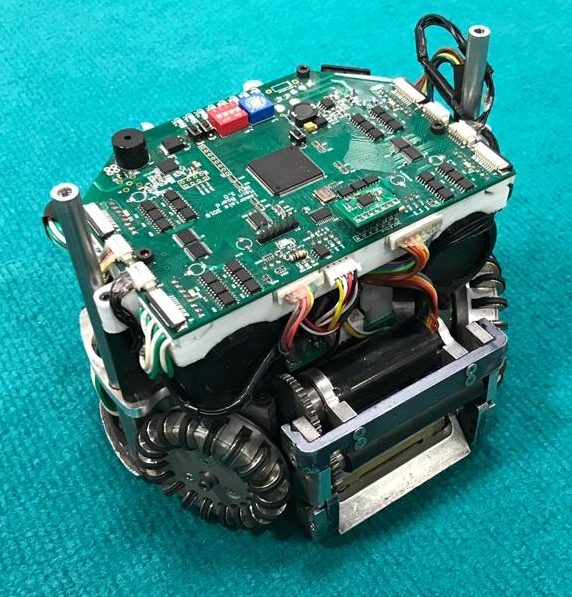
\includegraphics[width=\textwidth]{images/std_robot.jpeg}
         \caption{Standard}
         \label{fig:robot_std}
    \end{subfigure}
    \hfill
    \begin{subfigure}[b]{0.5\textwidth}
        \centering
        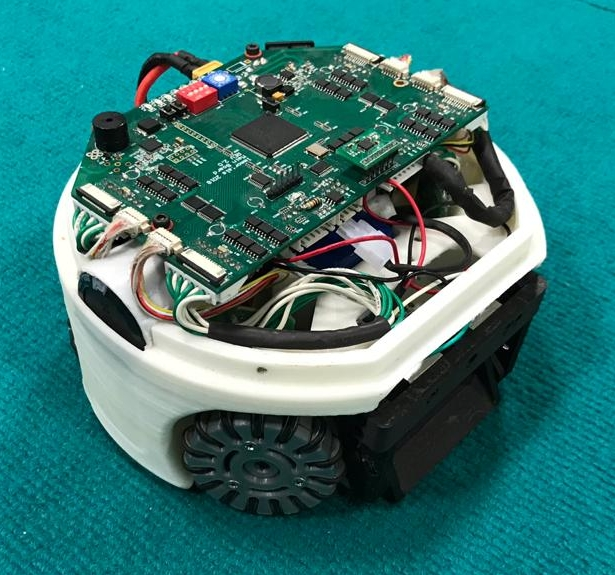
\includegraphics[width=\textwidth]{images/printed_robot.jpeg}
        \caption{3D-printed}
        \label{fig:robot_printed}
    \end{subfigure}
    \caption{Current Immortals robots}
    \label{fig:robots}
\end{figure}

\section {Mechanics}
In congruence with the mechanical design maintained from the previous year \cite{ref_ETDP2023}, the decision has been made to enhance the quality of 3D printing through the utilization of high-performance polymers, specifically Polyether Ether Ketone (PEEK). PEEK, renowned for its exceptional mechanical properties and resistance \cite{ref_peek}, presents an ideal candidate for elevating the performance and durability of printed components. The incorporation of PEEK into the 3D printing process not only promises heightened strength and resilience but also expands the realm of feasible applications, particularly in robust and reliable parts.

\section{Electronics}

\indent 
In the previous year, a comprehensive overhaul was undertaken to redesign all electronic components from the ground up, aligning with the latest advancements both within the specific league and the broader industry landscape. The primary objectives of this endeavor encompassed:
\begin{enumerate}
    \item[$\bullet$] reliability
    \item[$\bullet$] expandability
    \item[$\bullet$] being more competitive
\end{enumerate}

Following the composition of last year's Team Description Paper (TDP) and throughout the design and prototyping phases, several adjustments were implemented in the architecture, as depicted in Fig. \ref{fig:electronics-architecture}. These modifications, aimed at addressing previously encountered challenges, notably enhanced the functionality and performance of the system. However, it is imperative to acknowledge that these changes also introduced heightened complexity to the overall system architecture. Compounding this complexity was the global chip shortage, particularly affecting the availability of the Compute Module and other essential components. Consequently, despite the efficacy of the new designs, logistical constraints stemming from the chip shortage impeded the deployment of the updated boards on approximately half of our robotic platforms, deviating from our initial implementation plans.

All of our PCB and schematic designs are open-source and can be accessed on our GitHub page \cite{ref_github}.

\begin{figure}
	\centering
	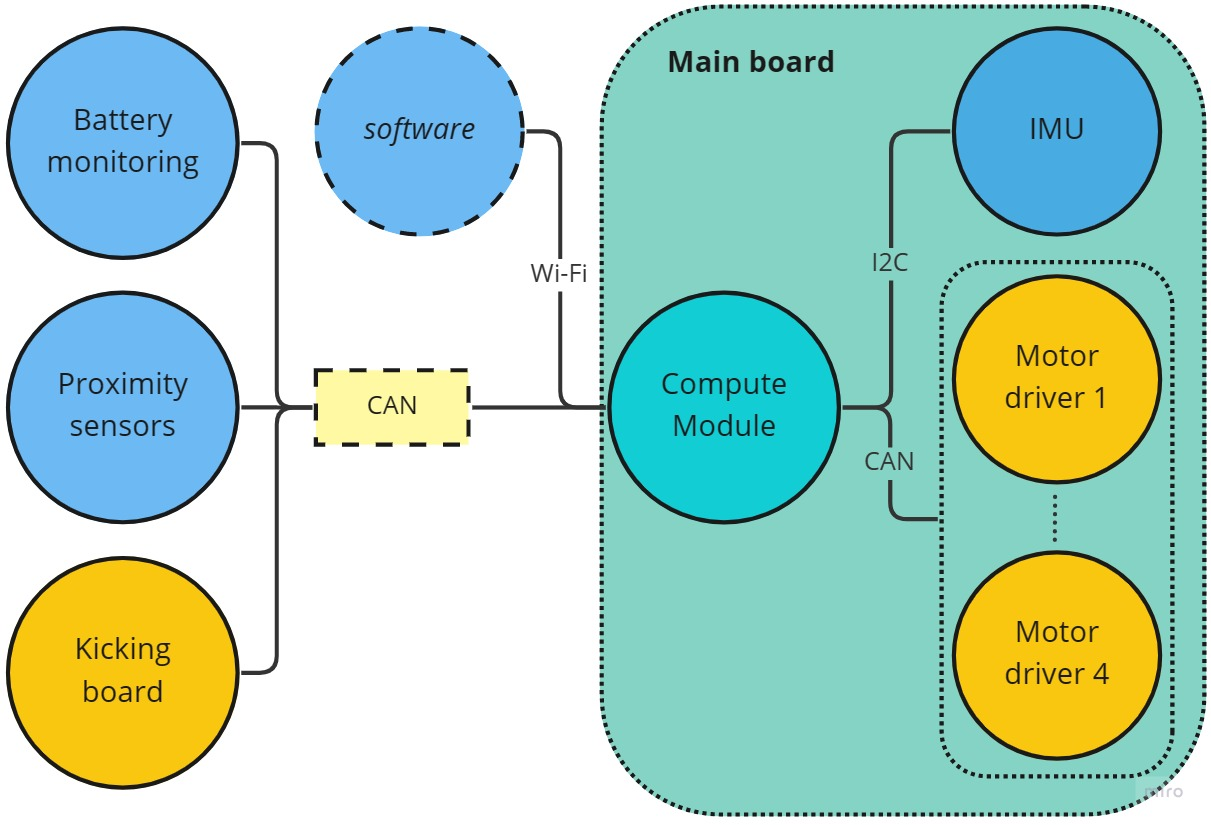
\includegraphics[width=0.8\textwidth]{images/electronics-architecture.jpg}
	\caption{Revised electronics architecture}
	\label{fig:electronics-architecture}
\end{figure}

\subsection{Main board}

Our current main board \cite{ref_mainboard} (as depicted in Fig. \ref{fig:main-board}) was meticulously designed and engineered during the previous year, integrating state-of-the-art components to optimize the performance of our robots. Central to its architecture is the utilization of the Raspberry Pi Compute Module (CM) 4, renowned for its computational prowess and versatility, serving as the cornerstone for local processing tasks within the robot. Furthermore, the design process involved meticulous consideration of various factors, including power efficiency, and compactness to ensure the optimal integration and functionality of the main board within our robot.

\begin{figure}
    \centering
    \begin{subfigure}[b]{0.45\textwidth}
         \centering
         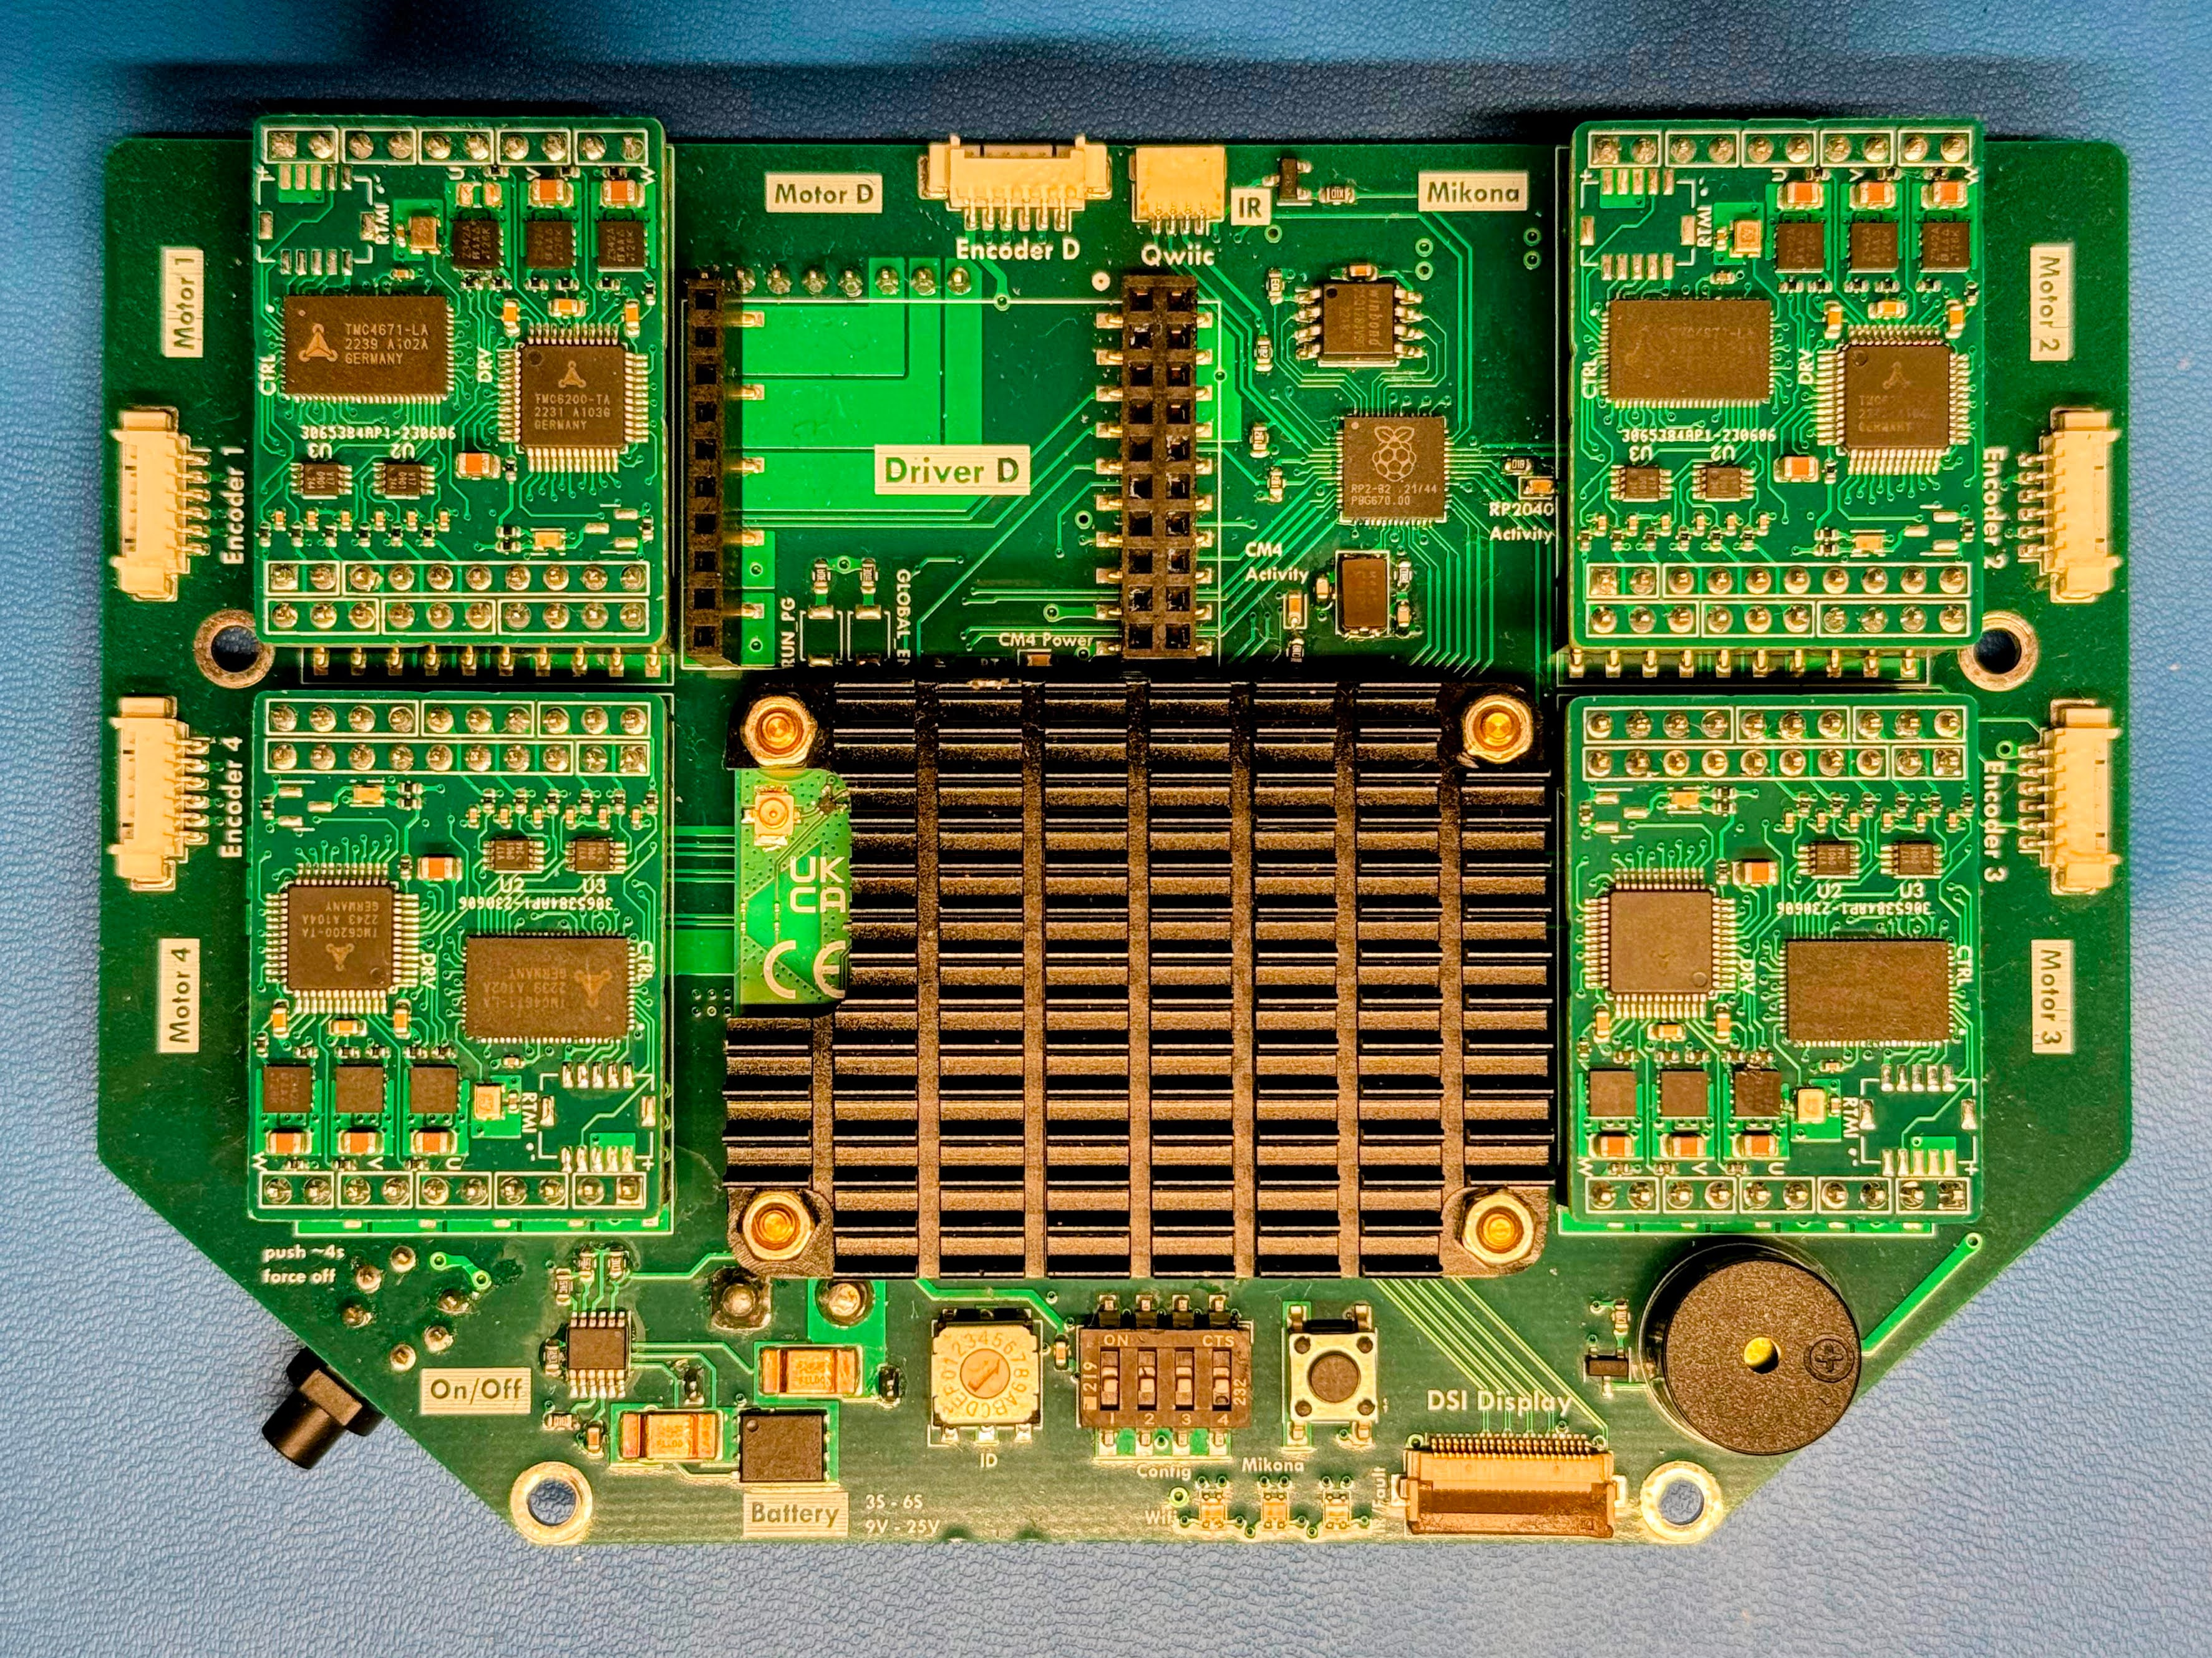
\includegraphics[width=\textwidth]{images/main-board.jpg}
         \caption{manufactured}
    \end{subfigure}
    \hfill
    \begin{subfigure}[b]{0.5\textwidth}
        \centering
        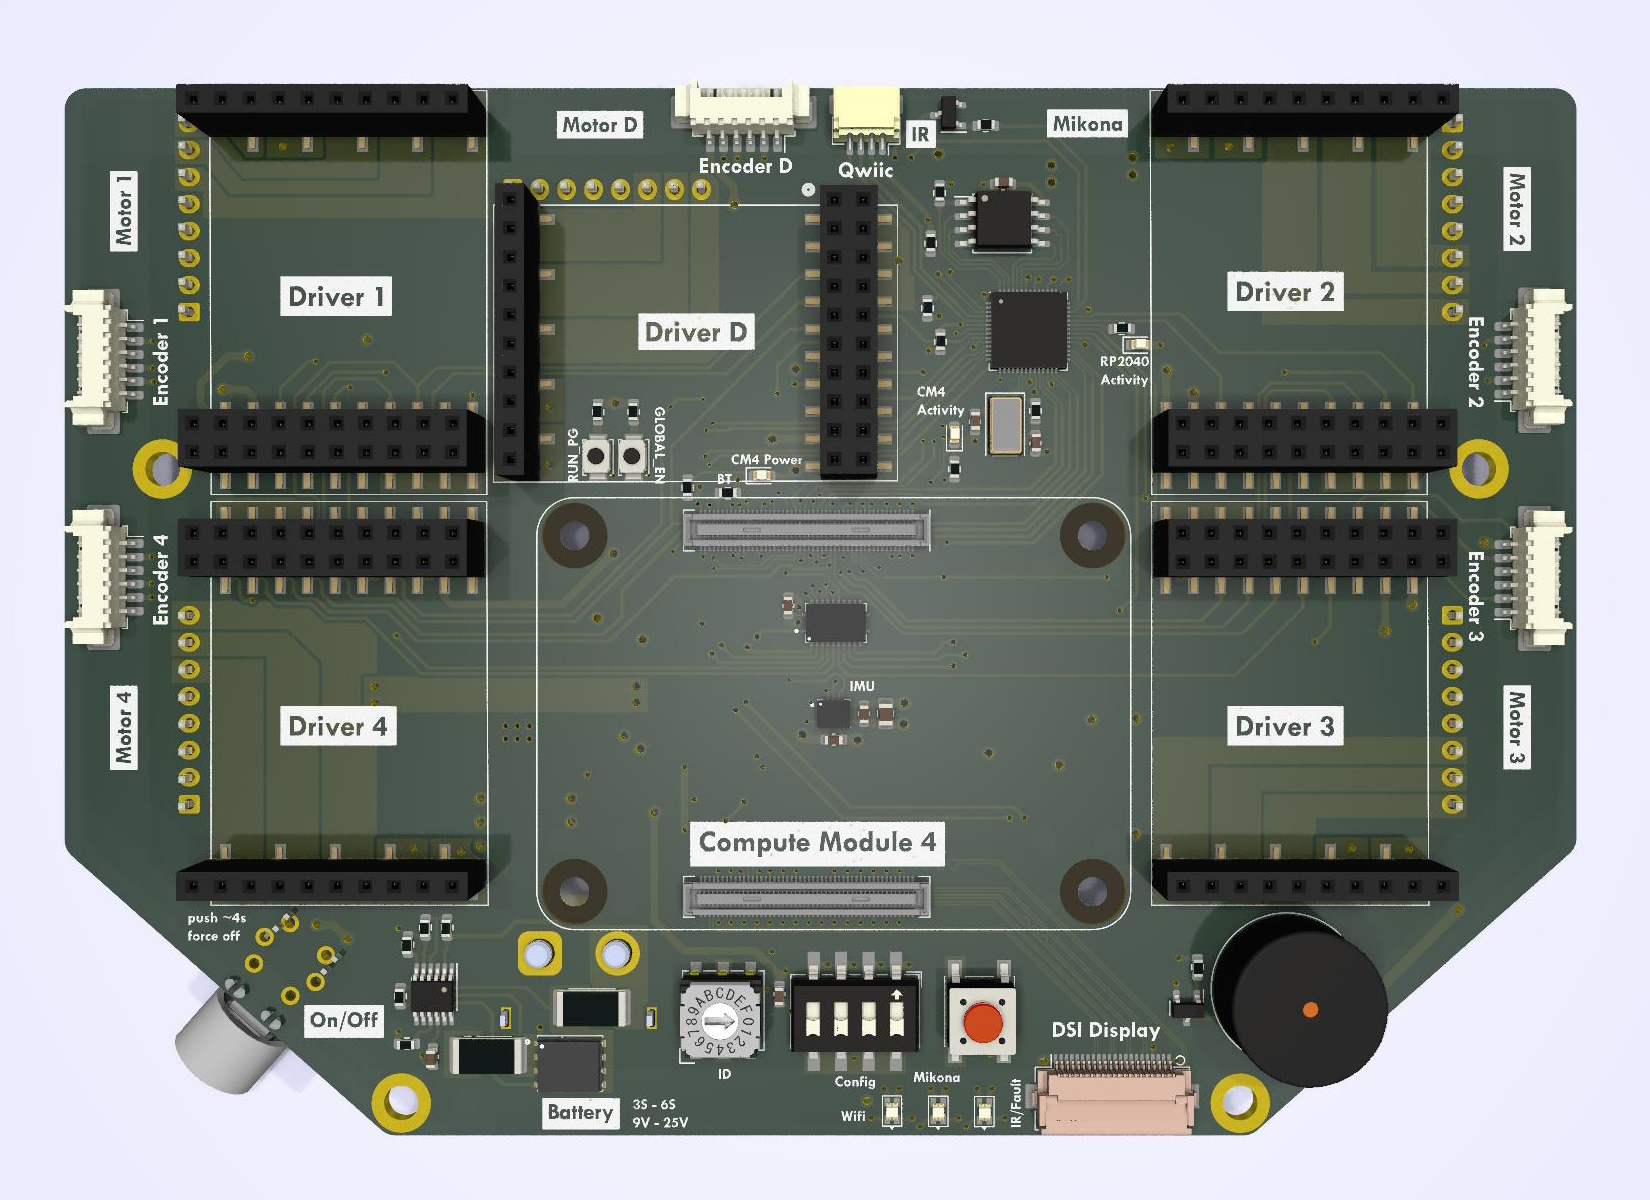
\includegraphics[width=\textwidth]{images/main-board-render.jpg}
        \caption{3D-render}
    \end{subfigure}
    \caption{The new motor driver module}
    \label{fig:main-board}
\end{figure}

In addition to the hardware advancements, the 5GHz WiFi band was employed as the wireless communication link between our server and robots. This decision was based on the positive experiences from the previous year's competition, where the use of 5GHz WiFi yielded results that were closely aligned with those obtained in controlled laboratory settings \cite{ref_ETDP2023}. The consistency and reliability observed under competitive conditions validated our choice, negating the need for an additional wireless communication system. Consequently, we decided against using an nRF wireless link, which, while offering benefits like reduced power consumption and potentially greater range, was considered superfluous given the effectiveness of our existing setup. This strategic decision not only simplified our system's architecture but also enhanced its reliability by minimizing the complexity and maintenance requirements associated with managing multiple communication protocols.

After evaluating our design as documented in last year's Team Description Paper (TDP), we made a significant change in our communication protocol with motor controllers, transitioning from the Controller Area Network (CAN) to the Serial Peripheral Interface (SPI). The primary motivations for this shift were the simplicity of the SPI system and cost considerations. Throughout the development and testing phases, the SPI bus demonstrated robust performance, and we did not identify any functional deficiencies that CAN might have addressed. Furthermore, the global chip shortage inflated the costs of CAN-compatible devices, compounded by the automotive industry's preferential access to these components, thus making SPI a more viable and economical option.

However, the implementation phase presented unforeseen challenges. We initially implemented the SPI communication using the built-in SPI driver in Linux, coupled with Trinamic's API. This setup, while functional, did not meet our performance expectations due to the slow operational speed. The integration involved sending each byte of data individually through the Linux kernel, resulting in a kernel mode switch with each transmission, which significantly hampered the speed and efficiency of data transfer.

In response to these challenges, we have adopted a manual implementation of the SPI bus for this year's competition. This approach allows for more direct control over the data transmission process and is expected to enhance the speed and reliability of communications between the Raspberry Pi and the motor controllers. We are currently conducting rigorous testing to validate this new implementation.

In addition to completely removing CAN from our system, we decided to adopt the I2C protocol for communication with various peripheral devices, including our battery monitoring system, proximity sensor (used for ball detection), and the kicking board. The choice of I2C was driven by its simplicity and efficiency in handling multiple short-distance communications.

\subsection{Motor driver}
In our current design, as depicted in Fig. \ref{fig:motor-driver}, the motor drivers are configured as separate modules \cite{ref_motordriver} that are mounted on top of the main board. This modular approach significantly enhances our ability to maintain and repair the robots, particularly in the event of motor driver failures. By isolating the motor drivers from the main board, we can quickly replace or repair a failed module without the need to dismantle other components, thereby minimizing downtime and improving the maintainability of our robots.
\begin{figure}
    \centering
    \begin{subfigure}[b]{0.45\textwidth}
         \centering
         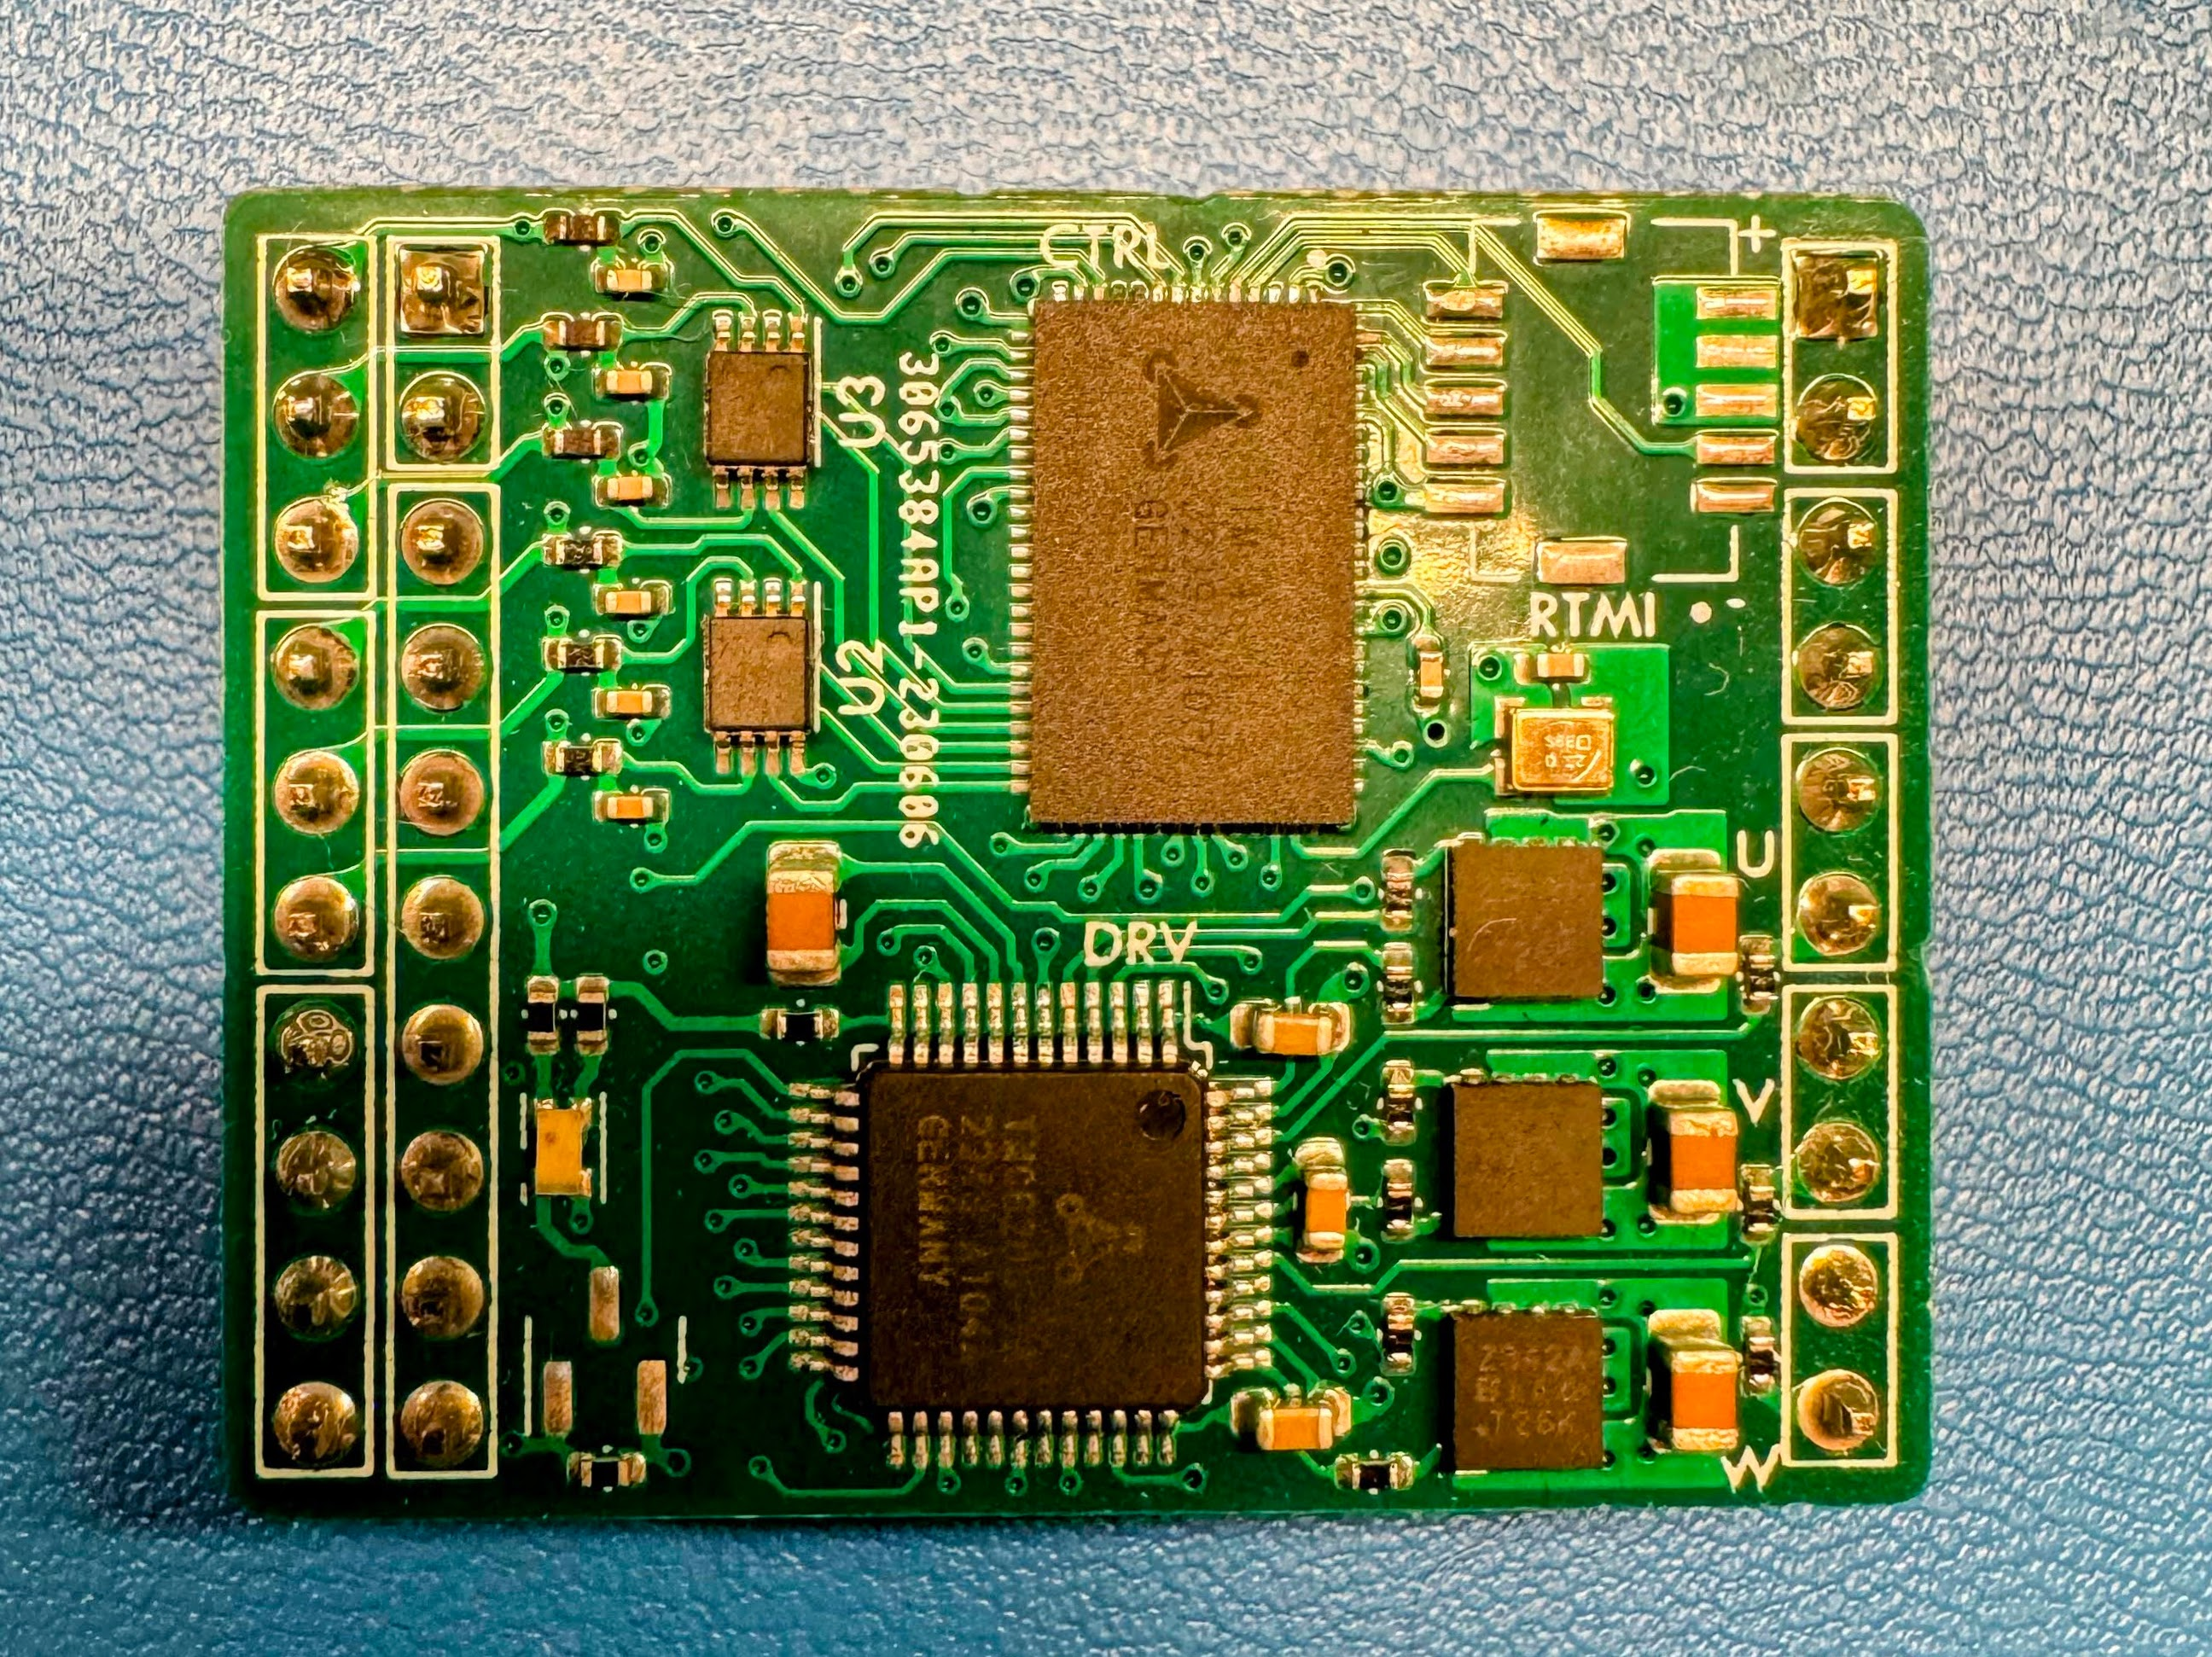
\includegraphics[width=\textwidth]{images/motor-driver.jpg}
         \caption{manufactured}
    \end{subfigure}
    \hfill
    \begin{subfigure}[b]{0.5\textwidth}
        \centering
        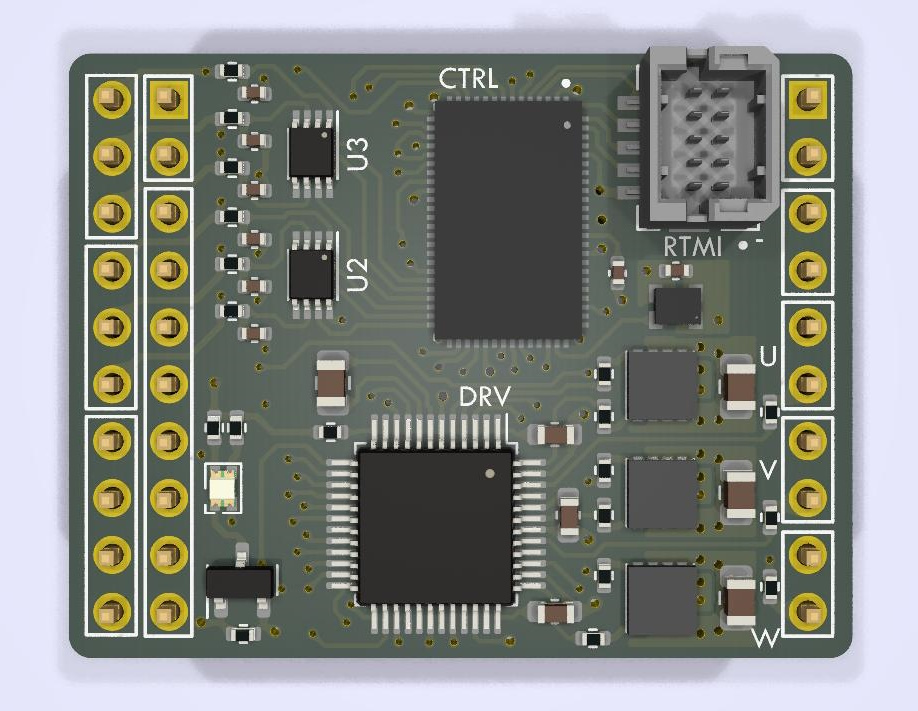
\includegraphics[width=\textwidth]{images/motor-driver-render.jpg}
        \caption{3D-render}
    \end{subfigure}
    \caption{The new motor driver module}
    \label{fig:motor-driver}
\end{figure}

We have integrated a dedicated BLDC motor driver IC, the TMC4671, into our system, which implements Field Oriented Control (FOC) for BLDC motors. This IC supports various control methods and offloads the local motor control functionality from the main processor to dedicated hardware. By doing so, it enhances the reliability of our system, particularly in terms of reducing latency and ensuring consistent performance under varying loads.

The motor drivers communicate directly with the Compute Module using the SPI bus. This setup facilitates a robust exchange of data, allowing the drivers to receive configuration settings and commands from the main processor and to send back vital sensor data, including motor speed and position. We utilize the Trinamic API, specifically designed for the TMC4671, to streamline the process of reading from and writing to the driver's registers, enhancing the efficiency of our control system \cite{ref_TMC_API}.

In addition to the TMC4671, our system incorporates the TMC6200 power MOSFET driver IC. This component is crucial for driving the MOSFETs used in our motor control setup and for sensing the motor currents that are essential for executing the FOC algorithm. The TMC6200 also includes an integrated fault detection mechanism, which is invaluable for maintaining the overall safety and reliability of the motor control system. It shares the same SPI bus as the TMC4671 and is directly connected to the Compute Module, ensuring that communication between these components is streamlined and effective.

Together, these components form a sophisticated motor control system that significantly enhances the operational capabilities of our robots, providing them with precise control and high reliability essential for competitive robotics.
\subsection{Kicking board}
In the design of our kicking mechanism \cite{ref_mikona}, as depicted in Figure \ref{fig:mikona}, we have integrated a dedicated LT3570 flyback capacitor charger IC. This component is specifically utilized to efficiently manage the charging of capacitors. The LT3570 IC is responsible for driving a BSC109N10NS3G MOSFET, which is connected to a DA2034 transformer within the circuit. This arrangement forms an essential part of the flyback converter system, designed to elevate the voltage to appropriate levels for rapid capacitor charging, essential for the operation of the kicking board.
\begin{figure}
    \centering
    \begin{subfigure}[b]{0.45\textwidth}
         \centering
         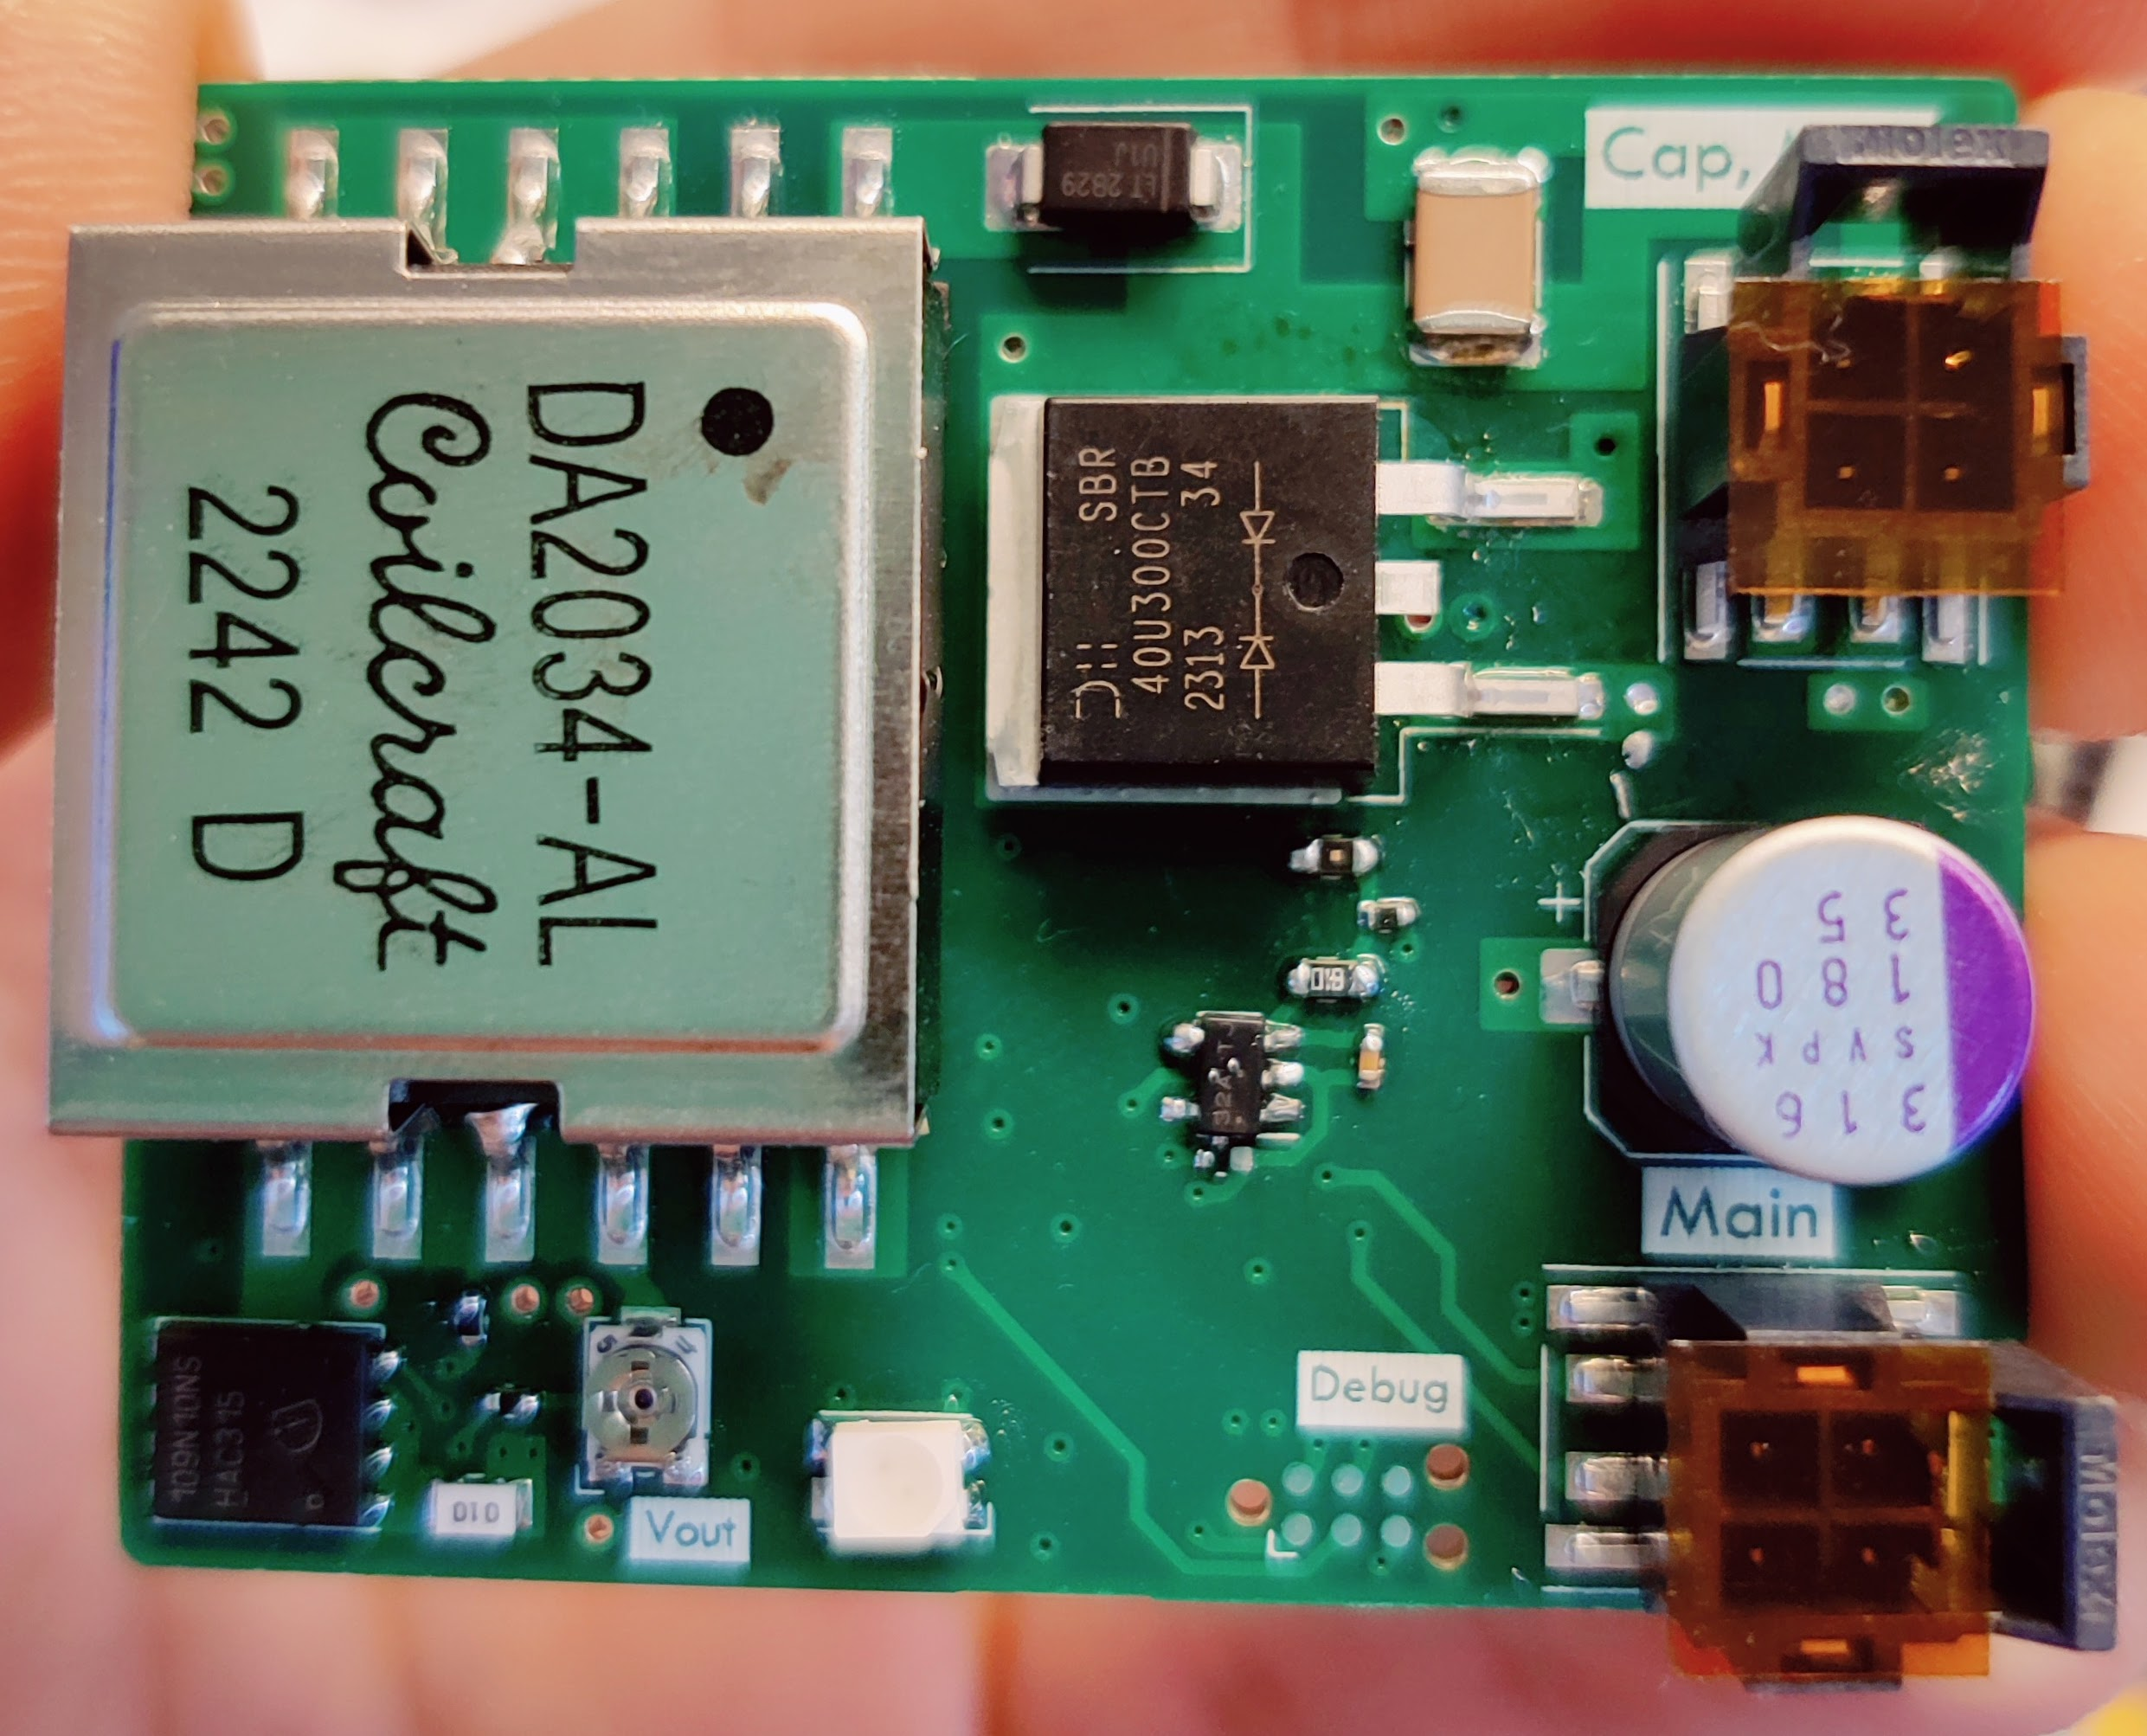
\includegraphics[width=\textwidth]{images/mikona.jpg}
         \caption{manufactured}
    \end{subfigure}
    \hfill
    \begin{subfigure}[b]{0.5\textwidth}
        \centering
        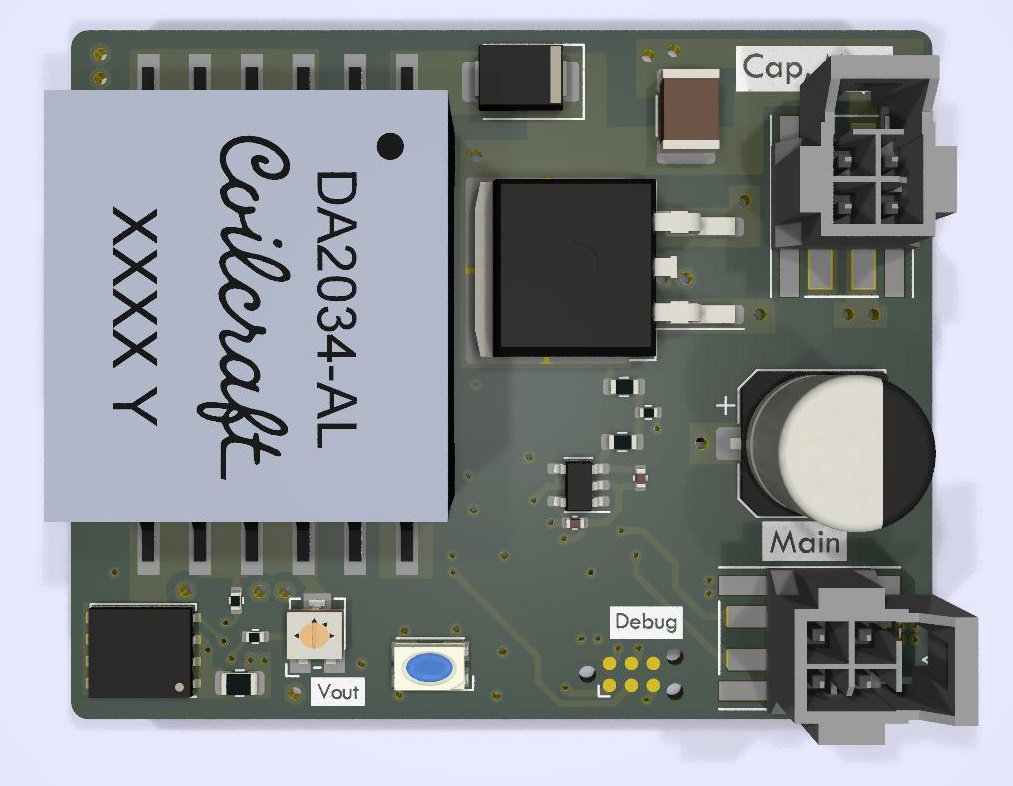
\includegraphics[width=\textwidth]{images/mikona-render.jpg}
        \caption{3D-render}
    \end{subfigure}
    \caption{The new kicking board design}
    \label{fig:mikona}
\end{figure}

Following the publication of last year's Team Description Paper (TDP) \cite{ref_ETDP2023}, we implemented a significant modification in our control system by transitioning from the STM32 microcontroller to a simpler PIC microcontroller. This change led to a substantial simplification of our circuit design, enhancing both the reliability and cost-effectiveness of our robot.

Additionally, our system incorporates a high-power resistor network, which is composed of three 2.4K ohm, 3W resistors. This network is specifically designed to safely discharge the capacitors as needed, independently of the kicker magnets. The discharge process is controlled by an STN3N40K3 MOSFET, which is driven by a ZXGD3009E6 driver, ensuring efficient and reliable management of the discharge cycle.

For the actuation of the kicking mechanism itself, two IGB50N60T Insulated Gate Bipolar Transistors (IGBTs) are employed. These are driven by a single IX4427MTR driver, which facilitates the rapid discharge of the capacitors directly into the kicking magnets, providing the necessary force for effective ball propulsion.

It is also noteworthy that the variable programmable resistor was removed from our system design after last year's TDP was documented. This decision was based on the finding that adjustments to the boost voltage were infrequently required. On the occasions where voltage adjustments are necessary, they typically coincide with hardware changes.
\subsection{Fault detection}

This year, we have implemented a significant improvement in our system's safety and reliability by integrating a separate microcontroller, the RP2040, specifically for detecting motor faults. The primary motivation for this change is to enhance the capability to rapidly identify any malfunctions in the motors or motor drivers. By doing so, we can immediately shut down the affected component before it has the opportunity to cause any damage to the main board.

The RP2040 microcontroller was selected for its high performance and efficiency in handling real-time processing tasks. It allows for continuous monitoring of the motor status. When a fault is detected, the RP2040 can execute a rapid response protocol, effectively disabling the faulty motor within milliseconds.

\subsection{Power management and monitoring}

This year, we have advanced our robot's power management system by implementing a sophisticated power monitoring and control system (Fig. \ref{fig:PMU}), moving away from traditional on-off switches. This new system incorporates an LTC2955 push-button controller and an LTC4231 micropower hot swap controller. These components work in tandem to enhance our power management capabilities, allowing for controlled power shutdown with a specific delay in the event of overcurrent conditions, without the need for traditional one-time fuses.

\begin{figure}
    \centering
    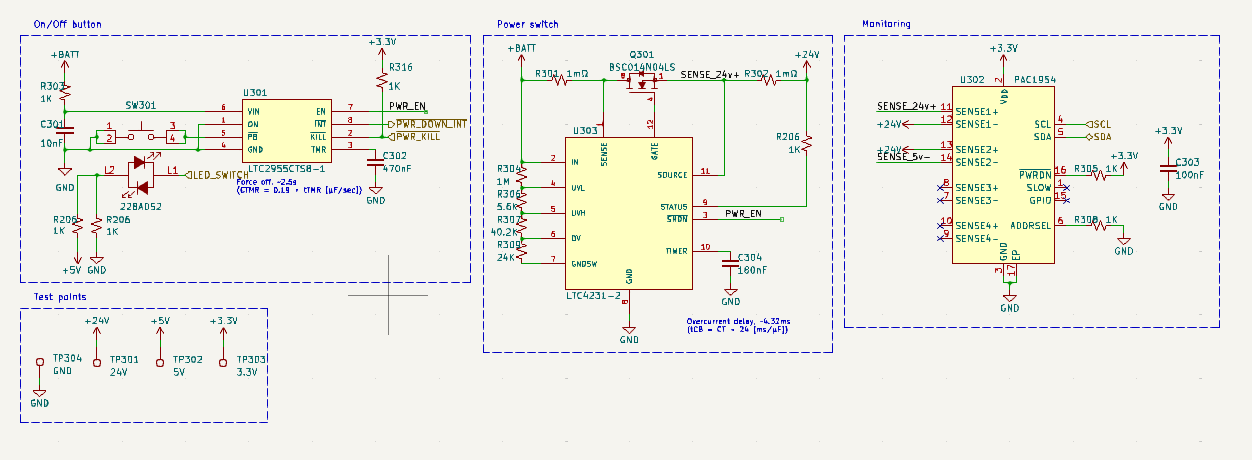
\includegraphics[width=1\textwidth]{images/PMU.png}
    \caption{Power management and monitoring}
    \label{fig:PMU}
\end{figure}

The LTC4231 plays a crucial role as a micropower hot swap controller, which allows for safe insertion and removal of boards in a live system. In our application, it helps manage the power distribution within the robot, particularly safeguarding against overcurrent scenarios. By monitoring the current flow and quickly disconnecting the power in case of an overcurrent, it prevents potential damage to the electronic components and the main board.

Additionally, we incorporated the PAC1954 current sensor to continuously monitor the battery's current.

\section{Software}
Last year we started to rewrite our software (Fig. \ref{fig:software-architecture}), focusing on the following points:

\begin{figure}
    \centering
    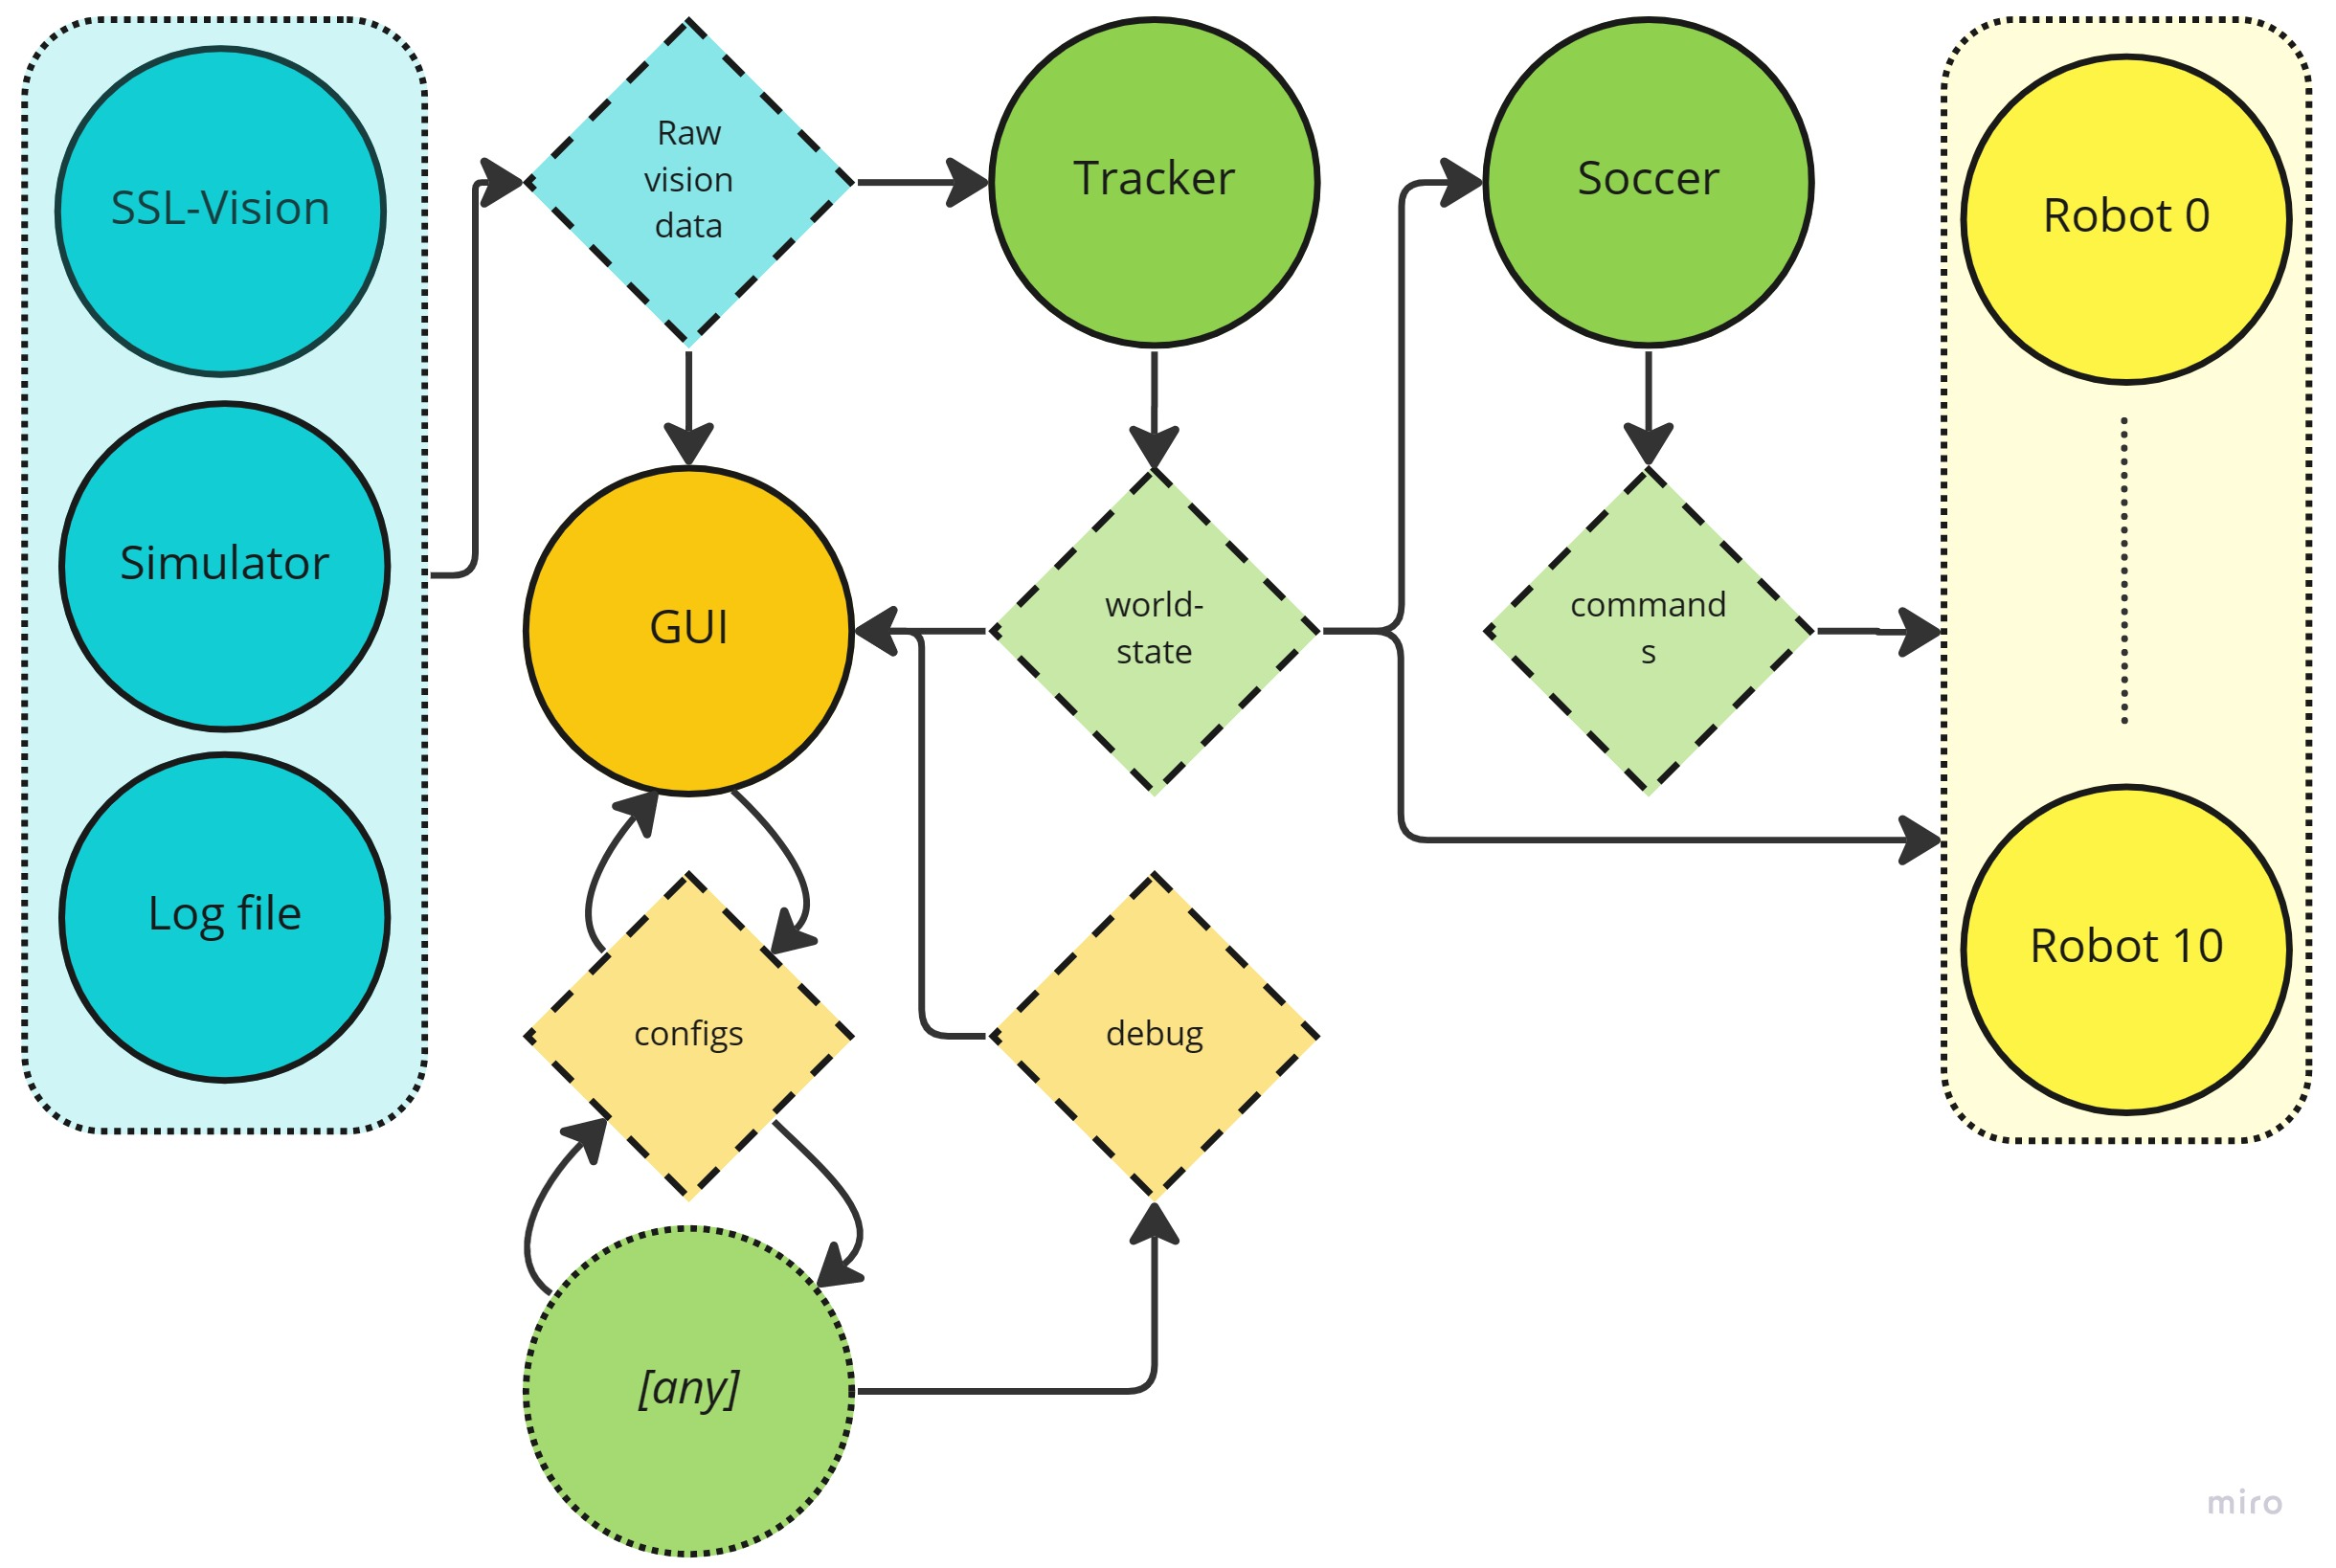
\includegraphics[width=0.8\textwidth]{images/software-architecture.jpg}
    \caption{The new software architecture}
    \label{fig:software-architecture}
\end{figure}

\begin{enumerate}
    \item more robust
    \item easier to read and understand
    \item faster to iterate and extend
    \item more competitive
\end{enumerate}

We managed to finish the rewrite and successfully test it in the simulator. However, using the new software during the real competition surfaced a huge number of issues. In the end we reverted to the old software, while cherry-picking parts of the development from the new rewrite.

In the following sections, we will describe the issues we faced, and ways we are planning to tackle them.

\subsection{Motion control}
Developing effective robot motion control systems presents a multifaceted challenge. This is especially true when relying only on simulated environments as test-beds. Our initial attempt at this endeavor encountered significant hurdles. These were primarily due to the inherent limitations of simulators. Simulators struggle to capture the complexities of real-world dynamics. They often fail to accurately represent the intricate interplay of physical forces. Also, they struggle with sensor noise and environmental uncertainties. These factors influence robot behavior. Controllers designed and optimized in simulation frequently falter when deployed on physical robots. This leads to suboptimal performance or outright failure.

In our previous endeavor, we faced the repercussions of this disparity firsthand. Despite promising results in simulation, our motion control algorithms proved ineffective when transferred to real robots, highlighting the inadequacy of our approach. However, rather than viewing this setback as a failure, we recognized it as an invaluable learning opportunity. Leveraging the data collected from our physical robots during last RoboCup, we gained valuable insights into the nuanced challenges and discrepancies between simulation and reality. This dataset, comprising observations of real-world interactions, sensor readings, and system responses, serves as a rich repository of information for refining our motion control strategies.

Building upon this foundation, our current approach integrates the lessons learned from our past shortcomings. We aim to develop motion control algorithms that are not only robust in simulation but also resilient in real-world scenarios. By incorporating the empirical knowledge gleaned from physical robot experiments, we seek to ensure that our controllers exhibit consistent performance across both domains. Through a data-driven methodology, we strive to create motion control systems that are adaptable, responsive, and capable of navigating the complexities of dynamic environments with precision and reliability.

\subsection{Alternative Programming Languages}
In our pursuit of refining our software, we recognize the pivotal role that programming languages play in facilitating efficient development workflows and minimizing error-prone coding practices. While C++ has traditionally served as a cornerstone language for robotics due to its performance and versatility, its stringent memory management requirements and relatively slow iteration times present significant drawbacks. Therefore, we are actively exploring alternative programming languages that offer enhanced development iteration and are more accessible to beginner programmers, while also mitigating the pitfalls associated with manual memory management.

A key criterion in selecting a new programming language is its ability to support hot-reloading, thereby enabling rapid iteration and experimentation without the need for time-consuming recompilation cycles. Hot-reloadable languages empower developers to make real-time changes to code and see immediate results, fostering a highly iterative development process that accelerates prototyping and debugging. This capability is particularly valuable in the context of refining robot motion control, skills, and plays, where quick iteration is essential for fine-tuning algorithms and adapting to evolving requirements.

Moreover, prioritizing ease of use is paramount, as it lowers the barrier to entry for novice programmers and streamlines the learning curve associated with robotics development. By selecting a language with intuitive syntax and comprehensive documentation, we aim to foster a more inclusive and accessible development environment, where individuals from diverse backgrounds can contribute effectively to our projects.

Furthermore, we seek a language that offers robust memory management mechanisms to mitigate the risk of common pitfalls such as memory leaks and segmentation faults, which are prevalent in C++ due to its manual memory allocation and deallocation model. A less error-prone language in this regard would not only enhance code reliability but also reduce development overhead associated with debugging memory-related issues.

Currently, we are actively experimenting with several candidate languages, including \textbf{\textit{Lua}} \cite{ref_3rd-lua}, \textbf{\textit{V}} \cite{ref_3rd-v-lang}, and \textbf{\textit{Odin}} \cite{ref_3rd-odin}, each of which offers unique features and advantages that align with our development objectives.

\newpage
\begin{thebibliography}{8}

\bibitem{ref_ETDP2023}
Immortals 2023 Extended Team Description Paper, \url{http://tinyurl.com/4xt23jb8}.

\bibitem{ref_github}
Immortals Open Source Project. \url{https://github.com/Immortals-Robotics}.

% 3rd-party libraries
\bibitem{ref_3rd-lua}
Lua, embeddable scripting language \url{https://www.lua.org/}

\bibitem{ref_3rd-v-lang}
The V Programming Language \url{https://vlang.io/}

\bibitem{ref_3rd-odin}
Odin Programming Language \url{https://odin-lang.org/}

\bibitem{ref_peek}
Kurtz, S. M., \& Devine, J. N. (2007). PEEK biomaterials in trauma, orthopedic, and spinal implants. Biomaterials, 28(32), 4845-4869.

\bibitem{ref_TMC_API}
The TMC-API is a portable C library for working with Trinamic ICs in embedded projects. \url{https://github.com/analogdevicesinc/TMC-API}.

\bibitem{ref_mainboard}
Immortals Open Source Main board \url{https://github.com/Immortals-Robotics/MainBoard}.

\bibitem{ref_mikona}
Immortals Open Source Kicking board AKA Mikona \url{https://github.com/Immortals-Robotics/Mikona}.

\bibitem{ref_motordriver}
Immortals Open Source Motor driver module \url{https://github.com/Immortals-Robotics/MotorDriver}.

\end{thebibliography}
\end{document}
